\section{Combustion Instabilities}

\subsection{Primary and Secondary Thermoacoustic Instabilities}

Combustion for engineering applications typically happens in systems of chambers, connected by long ducts. Although the chemical and hydrodynamic scales remain relatively short, and are localised to specific areas, e.g. the combustion chamber, acoustics travel throughout the system without significant damping due to the acoustically reflective materials used. Hence, the dominant acoustic eigenmodes of a system are therefore free to interact with the flame as they please. The resulting \emph{thermoacoustic} (TA) instabilities are classed as a form of chamber instability due to the reliance of the flame's spontaneous acoustics on specific geometries. The effect of thermoacoustics was first noticed in \cite{mallard1883RecherchesExperimentalesTheoriques}, where it was observed that flames can produce their own acoustic oscillations. Following this, \cite{rayleigh1896TheorySound} introduced a theoretical condition for a \emph{primary} TA instability, so called the \emph{Rayleigh criterion}, where fluctuations in pressure and heat release from the flame are amplified whenever they are in phase. To explain this in more detail, periodic changes to pressure are coupled to changes in acoustic velocity. This has a convective effect on the shape of the curved, hydrodynamically unstable \cite{darrieus1945PropagationDunFront,landau1944TheorySlowCombustion,matalon2018DarrieusLandauInstability} flames, resulting in an oscillation of the total heat release. This causes further oscillations to the radiated acoustic pressure from the flame, which closes this feedback mechanism. The primary TA instability can, hence, only occur when the oscillating pressure around the flames results in heat release oscillations which add to the acoustic pressure amplitude. Mathematically, instability is triggered whenever:
\begin{equation}
\rm{RI} \equiv \oint p' Q' \dd{t} > 0
\end{equation}
where $\rm{RI}$ is the \emph{Rayleigh Index}, $p'$ and $Q'$ represent fluctuations in the pressure and total heat release, respectively. The closed integral sign represents the integral over a single of the above mentioned periods. This statement translates to the statement that $p'$ and $Q'$ must be in phase with one another for instability to occur. This phase is controlled by the acoustics of the combustion chamber itself so small changes to combustor system's geometry can result in large qualitative changes to stability. When they are in phase, the feedback loop takes the form of a clockwise p-V cycle \cite{polifke2004CombustionInstabilities}, equivalent to an Otto cycle. This means the mechanism can generate mechanical work which, when confined to an engine, can take the form of a damaging force on engine parts, such as the damage observed in \cite{lieuwen2006CombustionInstabilitiesGas}.

Stroboscopic imagery of flames pro`pagating through tubes are shown in \cite{guenoche1964ChapterFlamePropagation} and made by periodically exposing the same film to the flame's light using a rotating drum. By establishing four different test configurations of these ducted flames (each of the two ends being either closed or open to the environment), the experiments establish flame structures common between these test cases. For one, all test cases have a flame which decelerates after ignition. They also observe oscillations in the flame's shape, not yet explained by the primary instability mechanism. These flame oscillations, \cite{guenoche1964ChapterFlamePropagation} concludes, are the result of the interaction of the acoustic oscillation of the gas, determined by the tube's acoustics, and the flame front.

\begin{figure}[t]
\centering
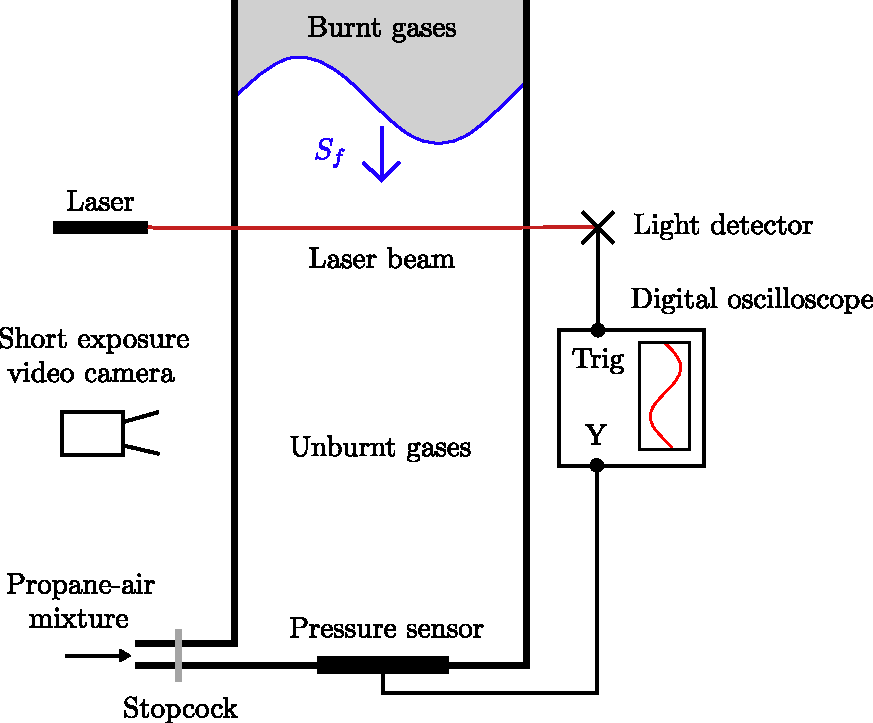
\includegraphics[scale=0.6]{assets/imgs/Searby-92.pdf}
\caption{Illustration of the experimental apparatus of \cite{searby1992AcousticInstabilityPremixed}.}
\label{fig:searby-experiment}
\end{figure}

An insightful experiment into thermoacoustics was performed later in 1992 by Searby \cite{searby1992AcousticInstabilityPremixed} and studied relationships between a cylindrical tube's acoustics as well as the speed and shape of the premixed flame within. The experimental apparatus is depicted in \fig{fig:searby-experiment}. Propane-air mixtures were lit at the top end of the tube and propagate down, with any acoustic disturbance detected by a pressure sensor at the bottom. Additionally, a small laser beam was place near the top of the tube to detect the flame as thermal gradients deflect the light. This triggers a digital oscilloscope to record pressure disturbances from the pressure sensor. A short exposure video camera was used to image the flame surface and observe its structure as it propagates. Since propane (C$_3$H$_8$) is a relatively heavy fuel with a species diffusion rate lower than methane's, the lean and stoichiometric mixtures used have Lewis numbers which are never below the critical Lewis number, $\Le_\rm{crit}$, required for \emph{thermodiffusive instabilities} \cite{zeldovich1944TheoryCombustionDetonation,barenblatt1962DiffusionalThermalStabilityLaminar,sivashinsky1977DiffusionalThermalTheoryCellular} to have an effect. Note that the downward propagating flames will have been somewhat stabilised by the \emph{Rayleigh-Taylor} (RT) instability. The primary instability is observed alongside a secondary, which is associated with a different feedback mechanism, acoustic envelopes and flame dynamics.

\begin{figure}[t]
\centering
\begin{subfigure}{0.49\textwidth}
\centering
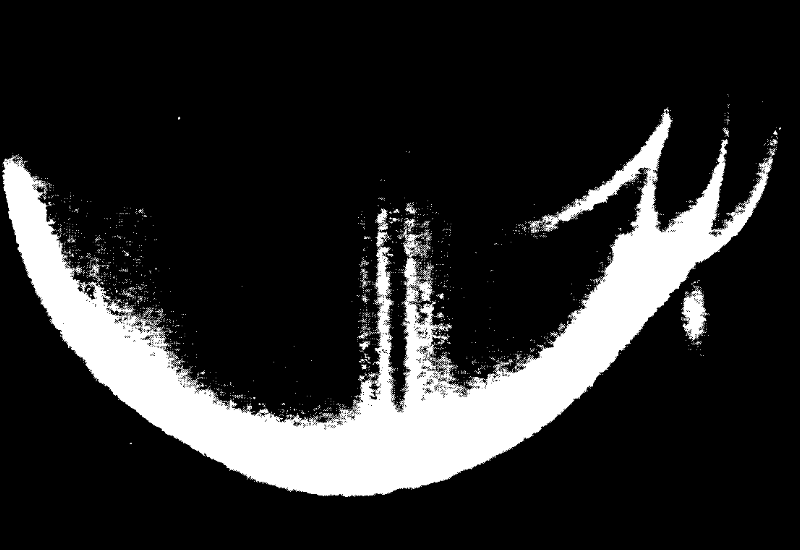
\includegraphics[height=5cm]{assets/imgs/Searby-92-flame_a.png}
\caption{}
\label{fig:Searby-92_flames_a}
\end{subfigure}
\hfill
\begin{subfigure}{0.49\textwidth}
\centering
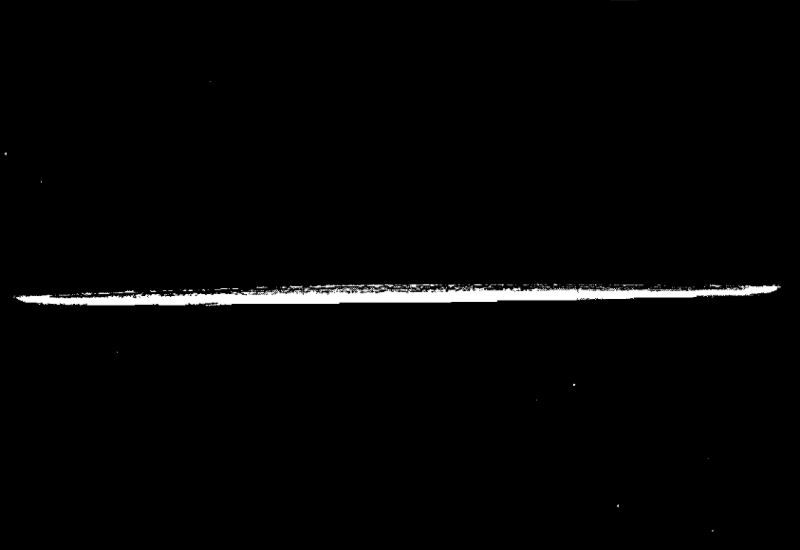
\includegraphics[height=5cm]{assets/imgs/Searby-92-flame_b.png}
\caption{}
\label{fig:Searby-92_flames_b}
\end{subfigure}

\vspace*{3mm}

\begin{subfigure}{0.49\textwidth}
\centering
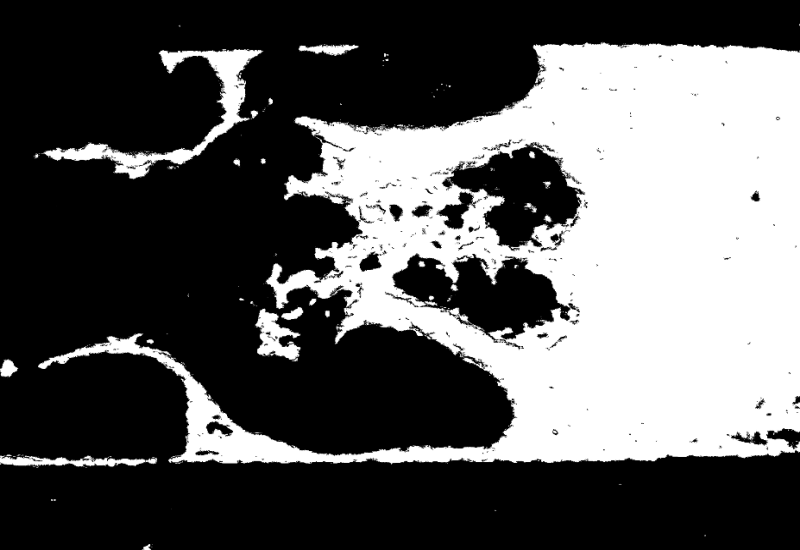
\includegraphics[height=5cm]{assets/imgs/Searby-92-flame_c.png}
\caption{}
\label{fig:Searby-92_flames_c}
\end{subfigure}
\hfill
\begin{subfigure}{0.49\textwidth}
\centering
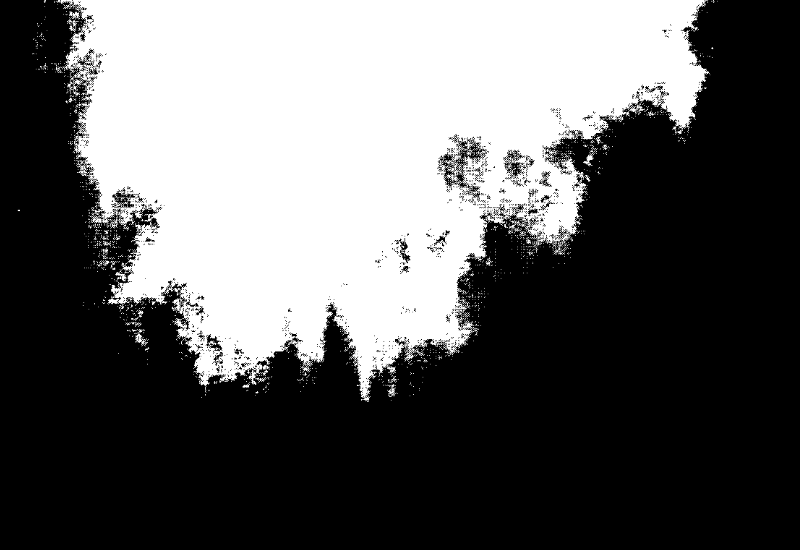
\includegraphics[height=5cm]{assets/imgs/Searby-92-flame_d.png}
\caption{}
\label{fig:Searby-92_flames_d}
\end{subfigure}
\caption{Photos, courtesy of \cite{searby1992AcousticInstabilityPremixed}, of flames at different stages of TA response. (a) shows the characteristic curved shape of a hydrodynamically unstable flame before any acoustics are significantly effecting the flame shape. (b) is a flame flame under the effect of the primary TA instability. (c) shows a cross-sectional slice of a flame rotated by $90\degree$ under the secondary instability. (d) shows a flame after the breakdown of cellular structures, which leads to a self-turbulent flame.}
\label{fig:Searby-92_flames}
\end{figure}

Initially, the flame curves as a result of the hydrodynamic instability, as photographed in \fig{fig:Searby-92_flames_a}. After some time, the acoustic amplitude increases due to primary instability. As the acoustic amplitude increases the flame flattens, seen in \fig{fig:Searby-92_flames_b}, resulting in a decrease in flame speed due to the decreased fuel consumption rate. In some of the flames tested, only the primary instability is observed, but in some others it progresses beyond this to the secondary instability -- often before the fully flattened flame is observed. At the immediate onset of the secondary instability, if it occurs, a cellular structure of a given wavenumber appears and corresponds to a rapid increase in the acoustic amplitude. This onset is much more rapid than for the primary instability, and eventually the cellular structure transitions into a symmetric flame structure similar to \fig{fig:Searby-92_flames_c}. Provided the flame has not yet reached the end of the tube it may also devolve into a self-turbulent flame similar to that shown in \fig{fig:Searby-92_flames_d}. The flame structures resulting from the secondary instability have significantly higher velocities as a result of their massively increased flame surface area and are viewed as a violent instability. The self-turbulent regime marks a significant decline to the acoustic amplitude as there is no regular release of pressure fluctuations from the flame.
% Flat flame under primary can be seen as a limit cycle

The secondary instability mechanism is seen by Searby \cite{searby1992AcousticInstabilityPremixed} as a \emph{parametric instability}. Searby and Rochwerger \cite{searby1991ParametricAcousticInstability} pose this system as a Mathieu equation by incorporating the effect of acoustic force into an equation for flame position under the influence of gravity, which is otherwise written as a damped harmonic oscillator \cite{searby1986WeaklyTurbulentWrinkled}. The Mathieu equation demonstrates a canonical example of parametric instability, since solutions remain unbounded whenever the forcing acoustic frequency is double that of the natural frequency implied by the flame in its damped harmonic oscillation. Physically this corresponds to a flame with a structure that oscillates with a period double that of the acoustic period.

% EXPLAIN WHAT S_L AND L_TH ARE
\begin{figure}[t]
\centering
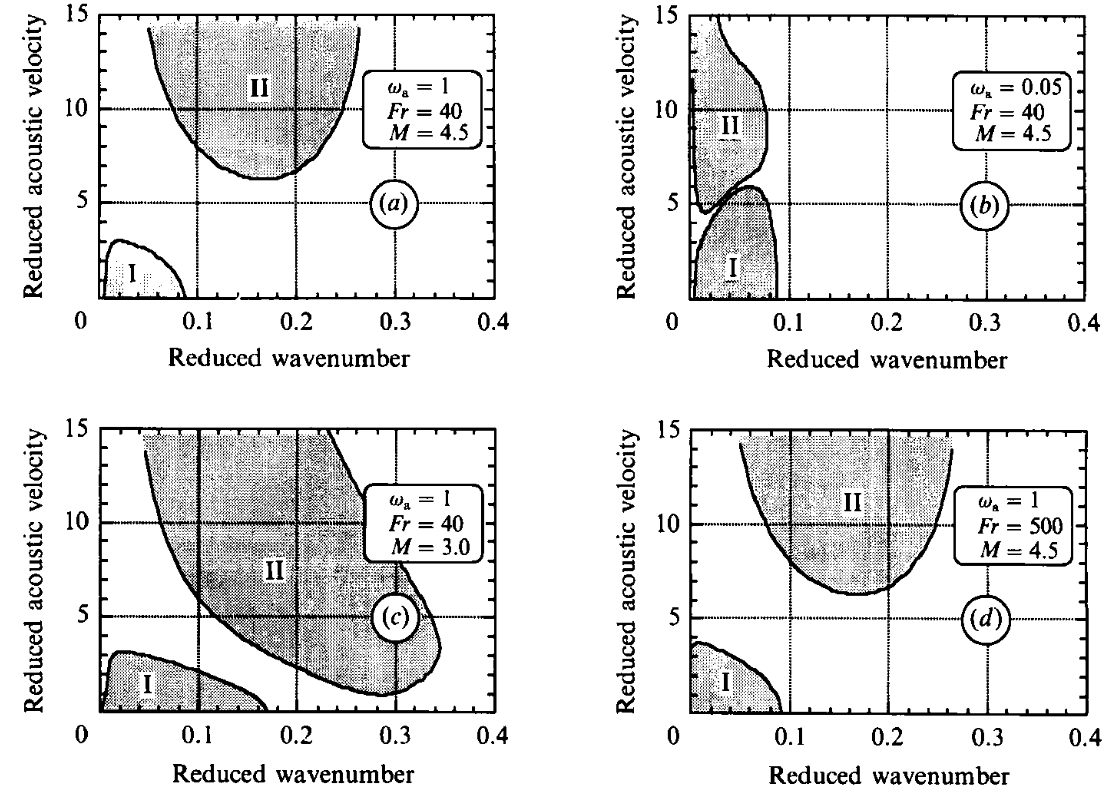
\includegraphics[height=11cm]{assets/graphs/thermoacoustic-stability.png}
\caption{Stability diagrams, courtesy of \cite{searby1991ParametricAcousticInstability}, for four different values of $ω_a$, $\Fr$ and $\Mk$. The regions I and II are regions of instability for the plane flame. Reduced wavenumbers are given as $k l_\rm{th}$ and reduced acoustic velocities are $u_a / S_L$.}
\label{fig:ta-stab}
\end{figure}

Using this formation of the flame front as solutions to the Mathieu equation, \cite{searby1991ParametricAcousticInstability} calculates regions of flame instability for a planar flame as functions of perturbation wavenumber $k$, acoustic velocity $u_a$ (the amplitude of which can be thought of as the intensity or volume of sound), acoustic frequency $ω_a$, Froude number $\Fr$ (representing non-dimensional inverse of gravitational forcing) and Markstein number $\Mk$ (a crucial flame parameter connecting the sensitivity of the flame's speed to perturbations to its surrounding hydrodynamics). They then plot these regions in \fig{fig:ta-stab}. Note that these plots do not acoustic instability mentioned above, but their effect on flame stability for a planar flame. In all the plots, there are two disjoint regions of flame instability. The region I represents hydrodynamic instability and occurs, as expected, at zero acoustic velocity for some wavenumber interval. This region ends at some finite $u_a$ as the primary acoustic instability eventually overcomes the hydrodynamic one. At non-zero acoustic velocity, region II of flame instability begins, corresponding to the aforementioned parametric instability. Interestingly, some of the graphs show acoustic velocities where regions I and II can coexist for different wavenumber intervals. In these cases, the primary thermoacoustic instability is expected to lead immediately into the secondary instability with no planar flame observed. On the other hand, for those acoustic velocities where neither region is present the planar flame is stable, so we see structures like \fig{fig:Searby-92_flames_b} where the flame has spontaneously flattened before any secondary instability can occur. We also notice that there is a wavenumber in region II which corresponds to the lowest unstable acoustic velocity. This means that once this acoustic velocity is met, only that wavenumber (and wavenumbers close to it) will be present as wrinkles in the flame. Finally, we note that the effect of increased gravity (decreased $\Fr$) on these downward propagating flames has stabilised the very low wavenumbers next to region I as the RT effect actually stabilises the plane flame.

An experiment was also performed by \cite{searby1991ParametricAcousticInstability} to demonstrate these results. A similar apparatus to \fig{fig:searby-experiment} was used, with significant changes being the usage of a loudspeaker in the bottom of the combustion tube to play sounds of wavelength one-quarter or three-quarters of the wavelength of the tube. A porous plate was placed above the loud speaker to remove any turbulence such that our laminar theories can be applied. Using the loud speaker to excite the flame at known volumes and frequencies (which correspond to controlling $u_a$ and $ω_a$, respectively), they observe both the planar and wrinkled flames described above. The sound intensity corresponding to the quietest parametrically unstable flame may then be plotted for a variety of acoustic frequencies, resulting in a curve predicted by the Mathieu equation model described above for a specific Markstein number. This enables the direct estimation of the Markstein number, which remains a difficult challenge and so remains a prevalent technique \cite{delfin2024ThermoacousticParametricInstability}.

% chaotic nature could be evidence of turbulence??
Beyond this, TA oscillations have been observed in a variety of experimentation. Methane-air combustion in a cylindrical tube was investigated experimentally in \cite{fichera2001ExperimentalAnalysisThermoacoustic} with data recorded from an optical sensor to detect changes to heat release, a pressure transducer for internal pressure recordings and a microphone for external pressure recordings. TA oscillations were observed and a non-linear analysis into the dynamical behaviour of the flame recordings demonstrate a chaotic nature to these thermoacoustics. The global stability of the flame, which is guaranteed by diffusive effects, is corroborated via calculation of the set of Lyapunov exponents. The thesis \cite{ebieto2017DynamicsPremixedFlames}, provides a detailed setup to gather high-speed imagery, chemiluminescent and pressure data in a variety of TA flames. The effects of a variety of phenomena affecting acoustic stability, such as RT instability, are outlined. Further experimentation is done on premixed flame oscillations in \cite{delfin2024VideoTransientParametric,martinez-ruiz2018VideoPremixedflameOscillations,delfin2024ThermoacousticParametricInstability} and provide high-fidelity imagery of flames under the effects of primary and secondary instability in \cite{delfin2024VideoTransientParametric,martinez-ruiz2018VideoPremixedflameOscillations}.





\subsection{Thermoacoustic Instability Modelling}

\begin{figure}[t]
\centering
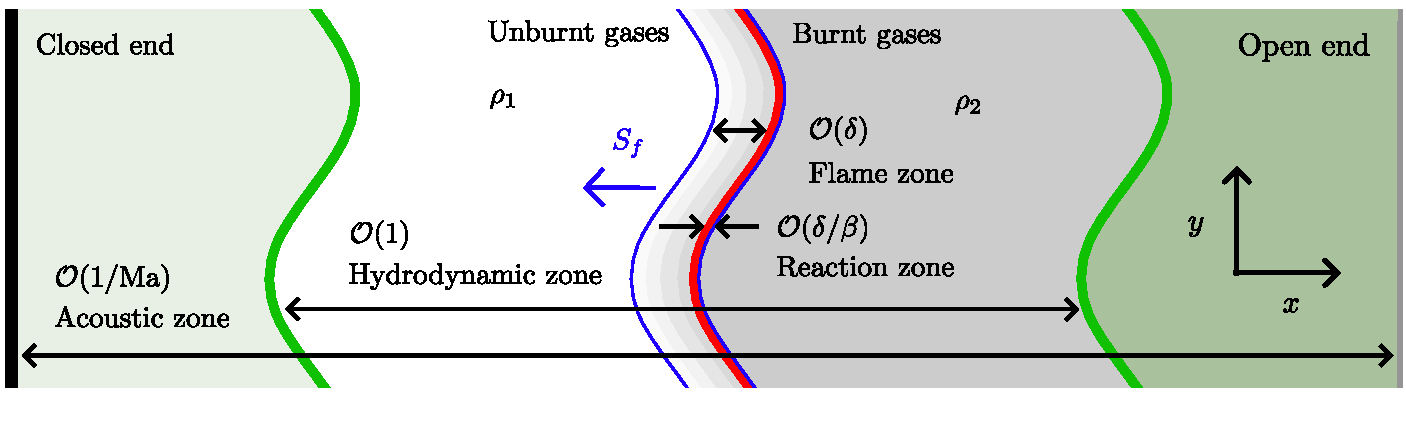
\includegraphics[scale=0.6]{assets/imgs/AW-flame.pdf}
\caption{Diagram showing the model geometry of the multiscale analysis performed by \cite{assier2014LinearWeaklyNonlinear}. The different non-dimensionalised asymptotic scales involved in the full analysis are labeled above the domain.}
\label{fig:AW-flame}
\end{figure}

Later on, work by Assier and Wu \cite{assier2014LinearWeaklyNonlinear} studied the stability of a \emph{flame-flow-acoustic} system, where a freely propagating flame in a closed-open, periodic duct is considered. \fig{fig:AW-flame} illustrates this geometry and is reminiscent of the experimental domain shown in \fig{fig:searby-experiment} of \cite{searby1992AcousticInstabilityPremixed}, excluding any wall boundary layer effects. Results from hydrodynamic flame theory \cite{matalon1982FlamesGasdynamicDiscontinuities,clavin1982EffectsMolecularDiffusion} are used to separate the dynamics within the flame from the outer fluid. This outer region is then separated into the usual $\cl{O}(1)$ hydrodynamic zone and a far-away $\cl{O}(1/\Ma)$ acoustic zone. Further asymptotic analysis is performed in the flame reference frame, coupling the two regions through dynamic jump conditions. A weak non-linearity assumption is made to simplify the flame equation such that linear stability analysis may be performed about the steady solutions to the Michelson-Sivashinsky equation \cite{sivashinsky1977NonlinearAnalysisHydrodynamic,michelson1977NonlinearAnalysisHydrodynamic,matalon2018DarrieusLandauInstability}.

They find that, when the acoustic interaction is included, these solutions are no longer linearly stable and the maximum growth rate of this instability increases significantly with heat release $q$. Non-linear stability analysis is also performed using a solver for the flame position coupled to the dynamical acoustic jump conditions. This is compared to the results of \cite{searby1992AcousticInstabilityPremixed} and they find they are able to qualitatively reproduce the primary instability and the onset of the secondary instability provided the flame parameter is allowed to deviate from its predicted value. In the latter case, the unsteady nature of the acoustic coupling to the flame induces an unsteady RT effect as the acoustic acceleration oscillates into and away from the less dense products. This is viewed as the driving mechanism behind this parametric instability. In a later conference paper, \cite{assier2014CombustionInstabilityModel}, tangential velocity terms are reintroduced and the parameter resulting in the same flame and acoustic behaviour as seen in \cite{searby1992AcousticInstabilityPremixed} more closely match the expected value. These results are surprisingly fruitful given they assume weak non-linearity in the face of the large heat releases the model is tested against.

In \cite{jun2023ParametricInstabilityPropagating} the secondary instability in hydrogen enriched methane-air flames is studied numerically in an open-ended tube. The structure of their flames under the full non-linear effect of the secondary instability is an impressive match to the experiment of \cite{ebieto2017DynamicsPremixedFlames}, in spite of a lack of convergence in the phase of sub-harmonic oscillations to the flame front (between grid spacings of 100 {\textmu}m to 50 {\textmu}m). They also find that the Rayleigh Index, $\rm{RI}$ is a good indicator for the onset of the secondary instability and that the violent acoustic output of this parametric instability may also be attributed to the changes in flame surface area strengthening oscillations in heat release which cause the thermoacoustic effect. They determine the main reason secondary instability is not seen in simulations of faster flames is simply that the tube is not long enough for the instability to develop before the flames reach the end of the tube. This validates a desire to model the behaviour of flames which are held in place, such as those in a held in place by combustor geometry in counterflow.


% veiga-lopez2020ThermoacousticAnalysisLean
% - Experimental study of H2-air flames in Hele-Shaw cells
% - Study effects of confinement due to cell geometry, gravity and mixture composition on thermoacoustic oscillations
% - Heat loss effects are most prevalent for very thin cells, where ...




\subsection{G-Equation Model}

% Aimee morgans




\subsection{Low-Order Thermoacoustic Modelling}

% n-tau models
% control theory stuff i don't understand

\cite{juniper2018SensitivityNonlinearityThermoacoustic}




\subsection{Instability Control}

\begin{figure}[t]
\centering
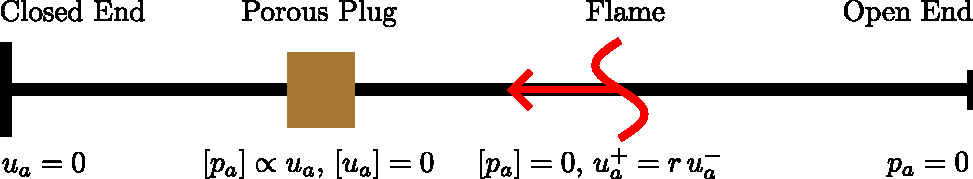
\includegraphics[scale=0.6]{assets/imgs/GP-model.pdf}
\caption{Illustration of the one-dimensional model considered by \cite{gaton-perez2025MitigationThermoacousticInstabilities}, where boundary conditions for each component of the model are shown.}
\label{fig:GP-model}
\end{figure}

Simpler analysis is performed by Gatón-Pérez et al. \cite{gaton-perez2025MitigationThermoacousticInstabilities} to evaluate the eigenstates of a one-dimensional closed-open tube containing a porous plug and a flame. Using Darcy's law to model the plug and assuming linear acoustics, the acoustic eigenmodes of the tube are found numerically. Experimental data is then compared against the one-dimensional model depicted in \fig{fig:GP-model}, where the heat release parameter, thermal length scale and the plug's permeability set by experimental values. Effects of heat losses through the combustor walls is given by \cite{flores-montoya2022NonadiabaticModulationPremixedflame}. The model is able to predict the flame locations within the tube which are most likely to trigger thermoacoustic resonance despite no consideration of the flame's motion or its thermal response to acoustics being made. These are the locations where the resulting acoustic eigenmodes have the lowest decay imposed by the porous plug. In this way, they show experimentally that the location of the porous plug may be chosen to preferentially mitigate different frequencies and reduce the likelihood of thermoacoustic instability. Evidently though, a simple one-dimensional model of this ilk is restricted in application to strongly one-dimensional, ducted combustors. As soon as a broader combustor or plenum is used, the two-dimensional acoustics (e.g. Helmholtz modes) must also be considered.

% luzzato2015ModellingControlCombustion (THESIS)

% liao2025ActiveControlThermoacoustic

% meadows2015PorousInsertsPassive

% mcmanus1993ReviewActiveControl




\subsection{Intrinsic Thermoacoustic Feedback}

\begin{figure}[t]
\centering
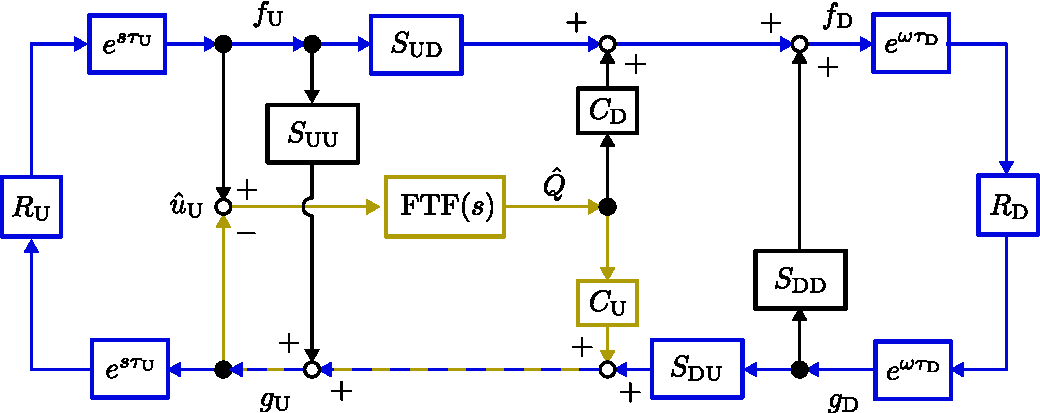
\includegraphics[scale=0.65]{assets/imgs/ITA-mech.pdf}
\caption{INTRINSIC THERMOACOUSTIC FEEDBACK LOOP}
\label{fig:ita-loop}
\end{figure}

% Doesn't need to be too elaborate!

% But there are not just acoustic modes, the full set of thermoacoustic instability modes includes ITA too [cite?]
% explain feedback loop
% phasors are cool
% some other stuff i read about
% cite the good reviews!

\cite{emmert2015IntrinsicThermoacousticInstability}
\cite{silva2023IntrinsicThermoacousticInstabilities}
\cite{hoeijmakers2014IntrinsicInstabilityFlame}
\cite{hoeijmakers2016FlameDominatedThermoacoustic}
\cite{orchini2025TrackingAcousticIntrinsic}
\cite{chen2024BiglobalLinearStability}
% Polifke?






\section[Computational Combustion Modelling]{Computational Techniques For Combustion Modelling}

\subsection{Computational Paradigms}

The combustion equations from \chap{ch:combust-model} are only analytically soluble in a limited number of contrived mathematical situations. For a general combustion initial value problem (IVP) then, computational methods are a requirement to approximate solutions to the relevant PDEs in a given domain, at some desired time $t$ after the initial conditions (ICs). To do this, approximation of derivatives in the time and space dimensions are separated into separate orthogonal problems, with different discretisations required in the temporal and spatial domains. We can then choose separately whichever temporal method, or time integrator, best fits the temporal problem alongside a suitable spatial method which is most appropriate for the expected spatial behaviour. A clear benefit of this numerical paradigm, then, is that problems like combustion which involve highly local phenomena (and excluding e.g. non-local gravitational effects such as those in astrophysical problems) allows the discretisation of the computation domain in space (referred to simply as the \emph{discretisation} henceforth) to many subdomains, split between different processing units, which interact only for discretisation points at the boundary between these subdomains. This \emph{domain decomposition} enables highly efficient distributed memory parallelism between many processors. The following discussion explores the two most popular paradigms for generating accurate spatial discretisation and the resulting logistics.

The most brute force way to simulate a fluid system would be one where you try to accurately simulate every detail involved in the fluid. This idea was first studied by Orszag \cite{orszag1970AnalyticalTheoriesTurbulence}, where he defines \emph{direct numerical simulation} (DNS) as a numerical simulation with enough grid points to full resolve the smallest physical phenomena in the system. Originally, Orszag studied this in the context of turbulent flows \cite{orszag1970AnalyticalTheoriesTurbulence,orszag1972NumericalSimulationThreeDimensional}. A turbulent incompressible flow is largely determined by the transit of its vortices, as expressed by the vorticity equation:
\begin{equation}
\pdv{\vb{ω}}{t} + (\vb{u} \cdot \vnab ) \vb{ω} = (\vb{ω} \cdot \vnab ) \vb{u} + \frac{μ}{ρ} Δ \vb{ω}
\end{equation}
where $\vb{ω} \equiv \vnab  \times \vb{u}$ and $\vnab  \cdot \vb{u} = 0$. Hence, turbulence is a fundamentally three-dimensional phenomenon -- the energy cascade from large to small vortices depends largely on the $(\vb{ω} \cdot \vnab )\vb{u}$ term above, which is not present for two-dimensional flows. In such flows, we have vortices not only on the order of the typical flow length scale $l_T$, called the integral length scale, but also of sizes all the way down to the smallest turbulence scale known as the kolmogorov length scale $l_K$ \cite{kolmogorov1941LocalStructureTurbulence}, where the rate at which viscous dissipation effects dampen vortices far exceeds the inertial forces of the vortex \cite{tennekes1972FirstCourseTurbulence,moin1998DirectNumericalSimulation}. In DNS of turbulent combustion, the smallest scale vortices must be resolved in addition to the smallest chemical length scales. In this context, the relevant time scales are chemical $τ_C = l_{\rm{th}} / S_L$, integral $τ_T = l_T / u'$ and Kolmogorov $τ_K = l_K / u'$ given an RMS velocity scale $u'$. Hence, the number of degrees of freedom required to resolve a three-dimensional box of size $L$ is \cite{domingo2023RecentDevelopmentsDNS}:
\begin{equation}
N_{\rm{tot}} = \left( \frac{L}{2 l_T} \right)^3 \Da \: \Ka \: \rm{Re}_T^{7 / 4}
\end{equation}
where we define the turbulent Reynolds number by $\rm{Re}_T \equiv ( l_T / l_K )^{4 / 3}$, Damköhler number by $\Da \equiv τ_T / τ_C$ and Karlovitz number by $\Ka \equiv τ_C / τ_K$. For typical turbulence intensities and combustion reactions, this results a discretisation length scale $δx$ on the order of 10-100 {\textmu}m. For example, in a simulation using $δx = 50$ {\textmu}m with a $10 \times 10 \times 10$ cm$^3$ computational domain, we require roughly 8 billion discretisation points. This workload is not only completely untenable for computation on personal computers, but remains prohibitive even for tier 2 High Performance Computing systems \cite{vlaamssupercomputercentrum2025TieringSystem,archer2020HPCEurope}, requiring resources usually available only at the national level. An example of this scale can be seen in the DNS of a real-size internal combustion engine in \cite{danciu2025DirectNumericalSimulation} -- large scale simulations of turbulent combustion are discussed further in \cite{chen2011PetascaleDirectNumerical}. Larger systems are needed not for their increased serial processing speed, but for the number of available processing units. Even excluding the potential for heterogeneous processing using GPUs, it is still only the largest supercomputers which provide the multiprocessing capability necessary to decompose such a large problem. Furthermore, regardless of the wall clock time taken to compute, it should be noted that any computation requires energy, so even after heavily parallelising the DNS roughly the same amount of overall energy is required (technically more due to the inefficiency in parallelising) to perform the full computation. Therefore, we should be careful of the cost in performing computational research in combustion to aid a clean energy transfer, when the cost requires the burning of fossil fuels.

Needless to say, the cost of simulation must be decreased before useful research may done. A simple way to do this is by modelling simpler physics in DNS than you know is present in the physical system. This is most effectively done by decreasing the number of species which are simulated, usually by removing minor intermediate species which are not a limiting part of the reaction mechanism. In so doing, the number of simulated differential equations goes down for each species removed -- if all species are removed besides product and reactant species, then only one mass fraction equation needs to be simulated. Further simplifications can also be made to the transport processes. But, one should note that benefits to accuracy in DNS are greatly undone when models are used which change the simplify the physical system. In any case, More efficient simulations may be used, which can be achieved by increasing the order of accuracy in derivative approximations. This is discussed in \sect{sec:high-order}.

To this end, another paradigm is often used for simulations, called \emph{Large Eddy Simulation} (LES) \cite{yang2015LargeEddySimulationPresent} where the same complex physics may be modelled with a coarser resolution. This relies on the use of a filtering technique called Favre averaging to remove \emph{subgrid scale} (SGS) turbulence smaller than a filter size $Δ$. This allows the discretisation length scale to be increased, so many fewer computations are required, especially in three-dimensions. The remaining kinetic energy is a vast majority of the kinetic energy in the system. The filtered motions must now be modelled. This is where the turbulence models are incorporated, usually consisting of a model for the SGS vortex viscosity values $μ_t$. In DNS of inert turbulence, the smallest length scale involved is the turbulent length scale, so the ratio of discretisation scales between LES and DNS, $Δ / δx$, is proportional to $(\rm{Re}_Δ / \rm{Re})^{3/4} = (u'_Δ Δ / S_L l_{\rm{th}})^{3/4}$, such that we have $N_{\rm{tot}, \rm{LES}} / N_{\rm{tot}, \rm{DNS}} = (\rm{Re}_Δ / \rm{Re})^{9/4}$ in three-dimensions, representing a massive reduction in computational cost \cite{pitsch2006LargeEddySimulationTurbulent}. The reduction in cost is obviously less so in two-dimensions, but this fine because two-dimensional flows are rarely as prohibitively expensive.

For LES of turbulent combustion, we have a much more complicated system \cite{veynante2002TurbulentCombustionModeling, pitsch2006LargeEddySimulationTurbulent}. Assuming our the shortest length scale at the flame is the chemical length scale $l_C$, then these filtered reaction terms must also be modelled at the flame. This poses an issue, since the vast majority of energy released from the combustion reaction happens on the smallest, chemical, length scales instead. In premixed combustion LES, this results in the introduction of several flame models for the turbulent flame velocity $S_T$ depending on the relative intensity of turbulence. Note that the combustion LES model used ought to account for the coupled effect of SGS eddies and combustion: reaction rates are modulated in premixed combustion by local thermal and molecular diffusion, which is aided by the turbulent mixing of the surrounding reactants. Most relevant engineering applications involve a level of turbulence corresponding to $\Ka > 1$, or the thin flame regime, although at Karlovitz numbers below one the weaker turbulence results in corrugated flames instead. At stronger turbulence intensities of roughly $\Ka > 100$, the reaction zones break into the broken reaction zones regime \cite{pitsch2006LargeEddySimulationTurbulent}. Depending on the relative size of filter $Δ$ used, the chaotic nature of the turbulence can result in qualitatively different behaviour -- exacerbated at high turbulence intensities.





\subsection{Spatial Discretisations} \label{sec:high-order}

\subsubsection{Traditional Methods}

Regardless of the paradigm used -- DNS, LES or Reynolds Averaged Navier Stokes (RANS), which is not discussed here -- numerically converged behaviour is only observed in a fluid simulation once a maximal discretisation length scale, $δx_{\rm{max}}$ is used. This corresponds to a minimum resolution required by the fluid simulation determined by the properties of that fluid, e.g. flame thickness, turbulence intensity, as well as the properties of the method used to perform the discretisation. Discretisations are most easily developed in one dimension. The canonical example of these are \emph{finite difference method} (FDM) approximations. The generic finite difference operator may be written as a weighted sum of differences. In one-dimension:
\begin{equation}
\dv{φ}{x} \Big|_i \approx L_x[φ]_i = \sum_{j \in \cl{N}_i} φ_{ij} w_{i, j}
\end{equation}
where $φ$ is the the function we have access to at points $\{\vb{x}_i\}_i$ and its derivative is represented by the finite difference operator $L_x[φ]$ at those points. At these locations, the surrounding points $\{\vb{x}_j\}_{j \in \cl{N}_i}$ are used to evaluate the differences $φ_{ij} \equiv φ_j - φ_i$ with weights $w_{i, j}$. These surrounding nodes are referred to as the \emph{stencil}. Centred finite difference approximations are FDM schemes where $\{\vb{x}_j\}_{j \in \cl{N}_i}$ is symmetric about the central node $\vb{x}_i$. These can easily reach high orders when uniform grid points are used and so reduce the required resolution mentioned above. The obvious caveat is that higher order methods always require more calculations, making each discretisation point in the domain essentially more expensive. But, this effect is usually dominated by the reduction in cost due to increased order of accuracy which improves the value of each discretisation point as the grid becomes more fine. Having said that, centred finite differences also suffer from stability issues because they are not upwinded for the hyperbolic waves. Accounting for this with one-sided upwinded schemes results in a compromise between stencil size and order. Compact finite differences solve the same linear problem, with the constraint that as few grid points be used in the stencil as possible [CITE]. In higher dimensions, finite differences are applied easily via a simple Cartesian product: to find $\vnab φ$ each partial derivative may be approximated by finite differences separately, provided the nodes are uniformly spaced in each dimension, creating a lattice. In three-dimensions, for example, this means we are restricted to modelling fluids within parallelopipeds (or cuboids assuming an orthonormal basis). Order (p-)adaptivity can be implemented simply by requiring different lattice points use different FDM schemes. Adaptivity in grid resolution (h-adaptivity) can be implemented by further subdividing parts of the lattice. This may also be used without adaptivity to better resolve parts of the computational domain, such as those close to the flame (e.g. the finite difference discretisation used in \cite{domingo2022RevisitingRelationPremixed} for a bunsen burner flame).

The AVBP solver \cite{cerfacsAVBP, schonfeld1999SteadyUnsteadyFlow} implements a Lax-Wrendoff formulation \cite{lax1960SystemsConservationLaws} -- as used in \cite{garby2013LargeEddySimulationCombustion} to model various combustor sizes, affecting acoustic properties. This is a form of non-method of lines finite difference scheme for hyperbolic PDEs where second order finite differences are used in space and time to reduce diffusive errors which erroneously smooth out linear and non-linear wave solutions. Secondary thermoacoustic instability structures of hydrogen-enriched flames are solved for in \cite{jun2023ParametricInstabilityPropagating}. In this case, the laminarSMOKE \cite{cuoci2013LaminarSMOKE, cuoci2013NumericalModelingLaminar} laminar flow combustion solver is used, which built on the popular CFD platform of OpenFOAM \cite{opencfdltd2004OpenFOAM, jasak2007OpenFOAMLibraryComplex, jasak2009OpenFOAMOpenSource} with combustion models supported by OpenSMOKE++ \cite{cuoci2015OpenSMOKE, cuoci2015OpenSMOKEObjectorientedFramework}. In this case operator splitting is used, such that second order central differencing is used for diffusive terms and second order upwinding scheme is used for convective terms.

% Maybe give some maths??
Another traditional class of discretisations are \emph{finite volume methods} (FVM). These are of relevance to any system determined by conservation laws as they enforce conservation by solving for the integral quantities of the problem (e.g. the integral quantity of density is mass). These integral quantities pass between different control volumes in the computational domain, as determined by the application of flux terms at their boundaries. This is important for combustion problems where the conservation of elemental mass, momentum and energy given in \sect{sec:govern} are the crucial physical constraints. The degrees of freedom are the centres of these volumes and smaller control volumes result in more accurate solutions, analogous to the grid points of FDM. Higher order FVM schemes are enabled using existing high-order quadrature rules to represent the relevant integrals [cite probably], although they are not as simple to implement as in FDM. Unlike FDM, the resulting mesh need not be rigidly uniform in each dimension, resulting in an unstructured mesh which can adapt to the problem -- especially useful for combustion systems. However, the reliance on a mesh to describe connectivity between volumes can be a major problem as low discretisation error is only guaranteed when a high-quality mesh is used. This is a major challenge for Lagrangian formulations of FVM [???].

Finite volumes are probably the most widely implemented discretisation method for fluid solvers by and large. One is implemented, for example, in the AVBP solver mentioned above. The PeleLM solver \cite{amrex-combustionPeleLM} also implements a finite volume discretisation of the low Mach formulation of the combustion equations -- that is, the equations in \sect{sec:govern} where acoustics are precluded. Examples of this being use in two- and three-dimensions are the thermodiffusive simulations of \cite{howarth2022EmpiricalCharacteristicScaling} and \cite{howarth2023ThermodiffusivelyUnstableLeanPremixed}. OpenFOAM \cite{opencfdltd2004OpenFOAM} implements a variety of discretisations, most notably a suite of finite volume methods, to a broad range of physical phenomena.

The \emph{finite element method} (FEM) is also commonly used to discretise fluid simulations. In this method, the computational domain is discretised into a mesh, like with FVM, except the discretisation points are located at the vertices of the mesh rather than inside the volumes they contain. Then, contributions to the overall solution are decomposed into many small contributions from each vertex by projecting the weak, integral form of the fluid problem onto finitely many small hat shaped elements. This results in a sparse linear problem describing the interaction of each element according to the equations, with non-diagonal matrix components resulting from local interactions. This decomposition onto a finite set of basis functions is referred to generally as a discontinuous Galerkin method \cite{zienkiewicz20051StandardDiscrete}. The simple, low-order connectedness in FEM allows for the mesh to change over time, making Lagrangian formulations natural. It is generally not used in a high-order formulation, however, with a typical scheme for fluid flow problems being second-order. Finite elements are used by \cite{camporeale2010FiniteElementMethod} to successfully recover the thermoacoustic instabilities of an annular combustion chamber. Its low order nature, though, means converged solutions are likely to contain large amounts of diffusive behaviour, especially in combustion problems where discontinuities are common.



\subsubsection{Less Traditional Mesh-Based Methods}

One high-order variation of FEM which is used to simulate combustion is the \emph{spectral element method} (SEM), which is used in the Nek5000 code \cite{nek1996NEK5000} [cite paper too] to discretise the combustion problem onto an unstructured mesh quadrilateral (two-dimensions) and hexahedral (three-dimensions) elements. In SEM. discretisation points are collocated onto nodes of the orthogonal Gauss-Lobatto (GL) polynomials within these elements such that the solution may be decomposed onto the corresponding GL basis \cite{patera1984SpectralElementMethod}. As a result, the order may be chosen arbitrarily by choosing the order of spectral GL polynomials and their corresponding node locations. This results in higher, often \nth{6} to \nth{10}, order discretisations at the cost of a much more challenging meshing problem due to the increased size of each element. The disparate effects of flame stretch and flame curvature on spherical flames are investigated using the Nek5000 code, for example \cite{giannakopoulos2015CurvatureMarksteinLength}.

A different approach is taken in \cite{krishnan2025NumericalMethodMultidimensional, patyal2018NonlinearDevelopmentHydrodynamicallyUnstable, creta2011StrainRateEffects}, where low Mach hydrodynamically unstable flames are modelled via a numerical discretisation of the hydrodynamic model for flames, rather than the full combustion equations. The hydrodynamic model \cite{matalon1982FlamesGasdynamicDiscontinuities,clavin1982EffectsMolecularDiffusion} splits the gas into two disjoint domains of hot and cold gas under the Navier-Stokes equations which are separated by an immersed boundary representing the flame. The flame is convected according to the Markstein model and boundary conditions over the flame are given in \cite{matalon1982FlamesGasdynamicDiscontinuities,clavin1982EffectsMolecularDiffusion} as an extension of the usual Rankin-Hugoniot relations. The computational domain is discretised using an \emph{essentially non-oscillatory} (ENO) scheme [CITE their one], which attempts to solve the typical issue of large oscillations at discontinuities like the flame by not interpolating over that discontinuity, similar to an upwinded FDM scheme. \emph{Weighted ENO} (WENO) improves on ENO by blending different interpolation schemes to improve its properties in smooth and discontinuous regions \cite{bozorgpour2025RecentAdvancementsFluid}. \cite{schuller2002ModelingToolsPrediction}, similarly, uses a WENO scheme coupled to a G-equation model for the flame to predict combustion dynamics of a bunsen burner flame. By comparison, WENO may also be used in simulations where the flame is not directly modelled, such as in \cite{berger2022IntrinsicInstabilitiesPremixed} where a third-order WENO scheme discretises the full combustion equations and is used to investigate intrinsic instabilities in flames.

A similar class of method are those which posses the \emph{total variation diminishing} (TVD) property. These more subtly reduces oscillations by ensuring the sum of variation of the dependent variables cannot increase between time steps. \cite{eigemann2025AmplificationThermoacousticFlame} investigates high-frequency noise using a TVD approach implemented by OpenFOAM.



\subsubsection{Mesh-Free Methods}


% Mesh free methods for combustion explored in \cite{kansa2009NumericalSimulationTwodimensional}, where they use RBFs
% Check Jack's paper for other examples of mesh-free combustion??

% SPH as precursor to LABFM
% \cite{monaghan1992SmoothedParticleHydrodynamics, vacondio2021GrandChallengesSmoothed}
% SPH is a mesh-free Lagrangian particle method* not used to simulate combustion and is rarely coupled to turbulence models due to its low order. It is a natural method to use in e.g. dam breaks and coastal applications where free surfaces are of interest. These free surfaces are not easily modelled by many other methods.
% It was found in [Steve's paper] that an Eulerian formulation of LABFM can be used to achieve high-orders provided you solve a linear system for each of the stationary particles as a preprocessing step [I SHOULD PROBABLY ACTUALLY READ THE PAPER THEN]



% LABFM is an Eulerian, mesh-free particle method inspired by this Eulerian form of SPH...





\subsection{Boundary Conditions}

\subsubsection{Inviscid Characteristic Boundary Conditions}

Usually, for reasons of computational cost, the geometry of a physical domain will not coincide with that of the computational domain. This is exacerbated when the physical domain is a theoretically unbounded. In such cases, it is necessary to truncate parts of the physical domain which are less important for the studied phenomena, so that computational expense may be focused. This process of truncation introduces boundaries to the computational domain which must allow for a physically reasonable and accurate interaction of it with the fluid. Often, for domains which are truncated we would like the boundary to offer some sort of non-reflection condition for waves which hit the boundary. For example, a transverse shear wave which reaches the edge of what is modelled of a semi-infinite duct would not physically reflect back at the truncated boundary. The same is especially true for acoustics, which will traverse the full combustor geometry the most frequently of all the waves. The same can also be said at computational boundaries not representing a truncated geometry: acoustic damping material in reactors may be used to diminish thermoacoustic instability and its non-reflectance must be modelled in the boundaries. The simplest boundary conditions (BCs) are those which simply prescribe values to dependent variables at the boundary discretisation points, e.g. $u, p = \rm {const}$, but these Dirichlet conditions fully reflect waves back into the interior domain. The same are true for Von Neumann BCs, where instead the derivatives of waves are full reflected. Instead, we may choose to model these characteristic waves directly through a \emph{characteristic boundary condition} formulation, such that waves which reenter can be directly prescribed.

% This is the basis of the \emph{Navier-Stokes characteristic boundary conditions} formulation, which does this by calculating 

% not just for this, we also need to apply BCs at walls
% !!!! The computational domain and physical domain usually do not coincide
% Many types of boundary conditions may be chosen for combustion schemes:
% - Periodic are very simple to enforce numerically so require no elaboration
% - No-slip or slip wall conditions
% - isothermal or adiabatic walls
% - acoustically reflecting or non-reflecting walls or inflow / outflow
% - In the case of inflow / outflow many more cases

A condition for non-reflecting BCs is first given in \cite{hedstrom1979NonreflectingBoundaryConditions} for the inviscid gasdynamics equations. It relies on performing a characteristic analysis by writing the one-dimensional, nonlinear, hyperbolic conservation equations in their primitive form, excluding source terms:
\begin{equation} \label{eqn:simple-hyp}
\pdv{\und{V}}{t} + \undt{\vb{A}} \pdv{\und{V}}{x} = 0
\end{equation}
($\und{V}$ is the vector of primitive variables and $\undt{\vb{A}}$ represents the `convection' of these variables by each other) and solving the left-eigenvalue problem of $\undt{\vb{A}}$ to find its left eigenvectors $\und{l}_m^T$. They then prove that enforcing the condition of $\und{l}_m^T \partial \und{V} / \partial t = 0$
gives precisely no waves entering the boundary in this continuous problem. The one-dimensional equation for acoustic non-reflection at a right-side boundary:
\begin{equation} \label{eqn:nonreflect}
\pdv{p}{t} - ρc \pdv{u}{t} = 0,
\end{equation}
is the basis of all non-reflecting characteristic BCs. Soon after, it was realised in \cite{rudy1980NonreflectingOutflowBoundary} that a perfectly non-reflecting boundary enables the pressure to drift arbitrarily, which means the mean pressure cannot be evaluated, leading to an ill-posed system. Naturally, this is a problem for any simulation subject to noise -- especially due to combustion noise \cite{dowling2015CombustionNoise} -- so they introduce a relaxation term in the form of a P-controller:
\begin{equation}
\left( \pdv{p}{t} - ρc \pdv{u}{t} \right) + σ(p - p_{target}) = 0.
\end{equation}
Then, the pressure relaxes towards a pressure $p = p_{target}$ provided the coefficient $σ$ is tuned correctly via linearisation of the fluid equations about a base state. Their following paper \cite{rudy1981BoundaryConditionsSubsonic} performs multiple tests on various inflow and outflow formulations therein. They conclude with the salient point that outflows are usually less sensitive to error in outflow data than inflows are to inflow data. They reason this as difficulties using their chosen extrapolation methods compounding (which would later become redundant), but may also be thought of with the simple idea that issues at an outflow are, usually, simply convected out of the domain whereas errors at inflow boundaries are spread throughout the domain.
% PLUS OR MINUS ρc IN THE ABOVE????? use only x direction!!!

Later on, a method to create characteristic BCs would be given in \cite{thompson1987LecturesSeriesComputational, thompson1987TimeDependentBoundary, thompson1990TimeDependentBoundaryConditions} which is the basis for many modern day non-reflecting boundary formulations. This method is referred to as the locally one-dimensional inviscid (LODI) approximation, since all diffusive and transverse terms are ignored. The approximation is explained in detail in \sect{sec:LODI}, but briefly: the same characteristic analysis is performed as above, except the hyperbolic equations are projected onto each eigenvector subspace $\und{l}_m^T$:
\begin{equation}
\pdv{\und{V}}{t} + \undt{\vb{A}} \pdv{\und{V}}{x} + \und{b} = 0
\quad \iff \quad
\und{l}_m^T \pdv{\und{V}}{t} + \cl{L}_m + \und{l}_m^T \und{b} = 0
\end{equation}
where $\und{b}$ holds source terms (e.g. gravity, chemical production rate) and $\cl{L}_m \equiv λ_m \und{l}_m^T \partial \und{V} / \partial x$. The eigenvalue $λ_m$ represents the speed of that characteristic. What's left, then, is to evaluate $\cl{L}_m$ for each characteristic variable at each characteristic boundary. This is elementary for waves which are leaving the domain, as the values may be evaluated from their definition via a one-sided FDM at the boundary which upwinds these outgoing waves. For incoming waves, however, these values must be modelled as we know nothing before making model assumptions about the waves outside of the computational domain. Several \emph{recipes} are then given in \cite{thompson1990TimeDependentBoundaryConditions} for non-reflecting inflows and outflows as well as several other conditions on these characteristics for wall boundaries and sub- and supersonic inflows and outflows.



\subsubsection{Viscous Reacting Characteristic Boundary Conditions}

Thompson's work would shortly after be extended to viscous flows in \cite{poinsot1992BoundaryConditionsDirect} -- that is, flows including parabolic terms associated with diffusion as well as the hyperbolic terms associated with waves. Previous paper show that theoretical well-posedness is ensured only when a total number of physical boundary conditions are applied, e.g. \cite{strikwerda1976InitialBoundaryValue}. This means that for inflows $5 + N_{\rm{S}}$ a total of physical BCs are required, and for outflows a total of $4 + N_{\rm{S}}$ physical BCs are required. Keeping count with the conditions already applied due to the LODI approximations, this means that one extra BC is needed at the inflow, and $3 + N_{\rm{S}}$ extra BCs are needed at the outflow. These new conditions are associated with the newly incorporated diffusive terms. At inflows normal gradients of normal stress are zero and at outflows normal gradients of tangential stress, normal heat flux and mass diffusion are zero. Mathematically, these are:
\begin{subequations} \label{eqn:znfg}
\begin{alignat}{3}
\text{At inflows:} \qquad &&
(\uvec{n} \otimes\uvec{n}) : (\uvec{n} \cdot \vnab ) & \bb{T} &&= 0. \\
\text{At outflows:} \qquad &&
(\uvec{n} \otimes \uvec{t}_{1 / 2}) : (\uvec{n} \cdot \vnab )& \bb{T} &&= 0, \\
&& \uvec{n} \cdot (\uvec{n} \cdot \vnab ) & \vb{\cl{E}} &&= 0
\quad \text{and} \\
&& \uvec{n} \cdot (\uvec{n} \cdot \vnab ) & (ρ \vb{V}_{\!α} Y_α) &&= 0
\quad \text{for } α = 1, \dots, N_{\rm{S}}.
\end{alignat}
\end{subequations}
It is shown in \cite{poinsot1992BoundaryConditionsDirect} that these diffusive conditions enable the stable and accurate simulation of time-dependent acoustics and shear phenomena travelling through these boundaries. Examples of vortices entering the domain for turbulence simulations would be left to later studies. In all cases of reacting flows, however, species have constant thermodynamic properties, severely restricting application of the method to idealised reactions. Later on, \cite{baum1994AccurateBoundaryConditions} would extend the LODI relations for reacting flows to multiple species of different molecular masses and gives numerical evidence of the boundary scheme being used to let a flame travel through the outflow boundary.

A note by \cite{nicoud1999DefiningWaveAmplitude} would then write the existing non-reflecting formulations of \cite{thompson1990TimeDependentBoundaryConditions,poinsot1992BoundaryConditionsDirect} as well as \cite{hirsch1990NumericalComputationInternal} and \cite{giles1990NonreflectingBoundaryConditions} which perform similar characteristic analysis to \cite{thompson1990TimeDependentBoundaryConditions,poinsot1992BoundaryConditionsDirect} which are equivalent to the non-reflection condition \equ{eqn:nonreflect} in one-dimension, but which do not coordinate in two-dimensions or higher due to transverse terms. This sort of comparative analysis is extremely valuable given the relative lack of work comparing a variety of methods. The AVBP solver \cite{cerfacsAVBP} is then used to perform quantitative numerical comparisons.

Following on from the pressire relaxation terms introduced by \cite{rudy1980NonreflectingOutflowBoundary}, it is pointed out in \cite{poinsot2001TheoreticalNumericalCombustion} that further P-controller terms may also be placed on velocity and temperature, at inflows rather than outflows, through the other characteristic waves. In so doing, the perfect reflection at these inlets is compromised to remove pressure drifting in the velocity and temperature values. This is especially useful in counterflow flames, where a drift in inlet velocity can lead to the flame leaving the domain. As with pressure relaxation, coefficients $σ'$ must be chosen via a linearisation procedure.

A unified formulation for non-reflecting boundaries is given in \cite{sutherland2003ImprovedBoundaryConditions} for viscous, reacting flows. This uses the LODI formulation from \cite{poinsot1992BoundaryConditionsDirect}, but includes source terms in \equ{eqn:simple-hyp} so strong local chemical effects are incorporated at these boundaries. Like \cite{poinsot1992BoundaryConditionsDirect}, they impose extra physical conditions on the diffusive terms, allowing for a smooth transition between inviscid solutions under the LODI approximations toward viscous solutions under the diffusive equations. Instead of the conditions \equ{eqn:znfg}, they use the conditions of \cite{dutt1988StableBoundaryConditions} which impose zero normal stresses etc. at the boundary rather than enforcing vanishing gradients:
\begin{subequations} \label{eqn:znf}
\begin{alignat}{3}
\text{At inflows:} \qquad &&
(\uvec{n} \otimes\uvec{n}) : & \bb{T} &&= 0. \\
\text{At outflows:} \qquad &&
(\uvec{n} \otimes \uvec{t}_{1 / 2}) : & \bb{T} &&= 0, \\
&& \uvec{n} \cdot & \vb{\cl{E}} &&= 0
\quad \text{and} \\
&& \uvec{n} \cdot & (ρ \vb{V}_{\!α} Y_α) &&= 0
\quad \text{for } α = 1, \dots, N_{\rm{S}}.
\end{alignat}
\end{subequations}



% Sutherland and Kennedy 2003
% - Provides a unified formulation for viscous, reacting flows
% - Uses the LODI formulation from P&L, but includes source terms so e.g. reaction terms at the boundary are included
% - Like P&L imposes extra physical conditions on the diffusive terms such that there is a smooth transition between inviscid solutions which use only the LODI conditions and variations thereof and viscous solutions
% - Suggests that a zero flux condition be rather than zero flux gradients, in accordance with [cite Dutt's paper]. Accordingly, zero normal stress is enforced at inflows and zero tangential stress and zero species diffusion is enforced at outflows.
% - They claim this allows a flame to travel through the outflow boundary, although the strong shear waves and tangential gradients imply that large inaccuracies should be present, whether or not the simulation remains stable
% - Are able to more accurately simulate flames passing through outflow boundaries, but find that the requirement of zero flux gradients in this case is a bottleneck to more accurate simulations of flame-boundary intersection


% Yoo and Im 2007
% - Propose improvements to the above scheme by shifting away from the LODI formulation by including tangential and viscous terms as well as the normal and source terms used in S&K
% - Impose physical diffusive BCs via zero flux gradients, unlike S&K
% - results in much improved results for flames passing through boundaries, especially in reproducing a more realistic circular flame shape 



%%% OTHER NON-REACTING FLOW STUFF

% Prosser 2005
% - performs asymptotic analysis in the low Mach formalism to make improvements to subsonic turbulence interactions with characteristic inflows and outflows
% - Working with the LODI assumptions does nothing to account for transverse effects like the convection of vortices over the boundary and hence results in spurious pressure oscillations when applied to turbulent flows.
% - For their non-reflecting turbulent inflows, for example, they calculate the incoming amplitudes of characteristic waves under turbulence relative to a \emph{frozen} turbulent solution rather than a quiescent flow


% Polifke 2006
% - investigates true reflection coefficients for non-reflecting outflows prescribed by Poinsot and Lele [cite] (includes a corrective P control term) over a range of acoustic frequencies and finds that arbitrarily low frequencies have R arbitrarily close to one
% - This fully reflective behaviour for low frequencies is restored by introducing a new term into the P controller 'relaxation' term which specifically masks plane waves at those low frequencies


% Prosser 2011
% - Can be seen as a counterpoint to YI2007 which extends his earlier work to boundary conditions for subsonic reacting flows


% Guezennec and Poinsot 2009
% - They find that the usual method of assigning L values at the boundary under the NSCBC formalism cannot be used to inject turbulent vortices at the same time as eliminating acoustic reflections
% - They propose a corrected method which again references a frozen turbulent flow VFCBC and results, practically, in halved L_5 values at inflows


\subsubsection{Immersed Boundary Methods}


% Immersed boundary methods are also an option and open up possibilities for boundaries not restricted specific node placement, especially for moving boundaries. But as detailed in King 2022, these a largely restricted to lower order accuracy at these boundaries (cite, and for what reason?).

% Although they are widely used in non-reacting problems, they are rarely used in combustion problems
% Matalon uses them in his hydrodynamic combustion solver!




\subsubsection{Delayed-Time Domain Impedance Boundary Conditions}


% Describe TDIBC briefly before going into time delay model!


\begin{figure}[t]
\centering
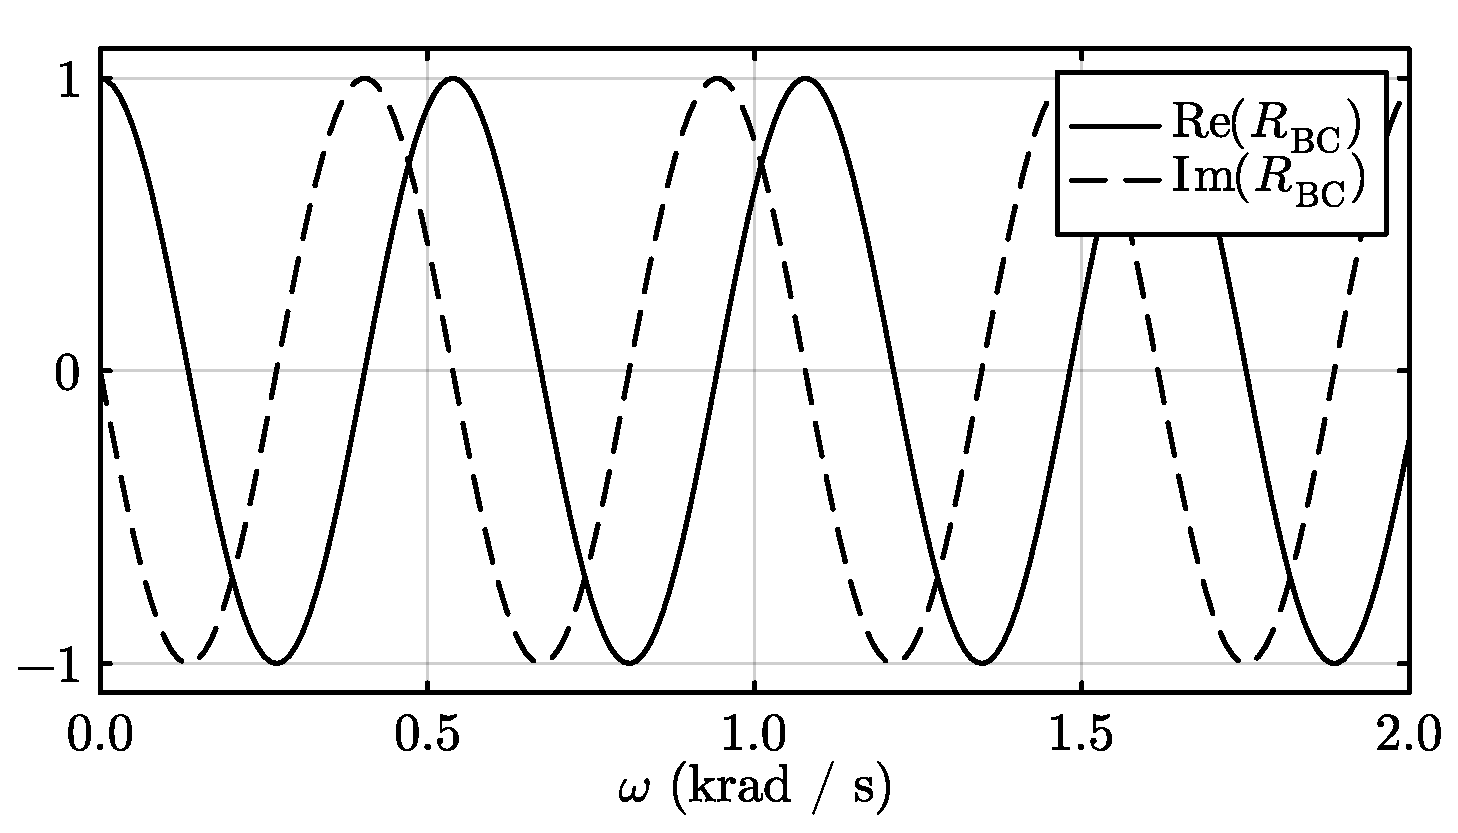
\includegraphics[scale=0.35]{assets/graphs/complex_R_Moire.pdf}
\caption{MOIRE PATTERN}
\label{fig:moire}
\end{figure}

Although many variations on TDIBC exist, the \emph{Delayed-Time Domain Impedance Boundary Conditions} (D-TDIBC) of \cite{douasbin2018DelayedtimeDomainImpedance} are particularly relevant for the simulation of thermoacoustic instabilities. By modelling the effect of an acoustic time delay, $τ$, a part of the computational domain -- say, an exhaust pipe -- may be truncated in place of a numerical boundary. Then, the response of this new boundary to incoming acoustics should be a sinusoidal Moiré pattern in the frequency domain, as shown by \fig{fig:moire}. The proposition of \cite{douasbin2018DelayedtimeDomainImpedance} is that this pattern may be modelled via a meromorphic function of $2n$ simple poles. The location of these poles and their residues are then found in a preprocessing step as the values which minimise the least-squares fit with the desired response curve. Each time step then, the resulting constants are used to evaluate the change in acoustic variable at the boundary in such a way that no memory of previous time steps are required. 

After validating the model by testing its response to a Gaussian pressure bump, the model is compared against DNS of methane-air combustion in a 2D flame holder, where the upstream end is closed and the downstream end is open. Comparing this to DNS where the last 25 cm at the downstream end has been truncated to use D-TDIBC, they find that the time delay model accurately recovers the one-, three- and five-quarter eigenmode shapes, with small quantitative errors in their sound spectra. Considering the $\sim 13\%$ reduction in degrees of freedom in the computational domain resulting from the truncation, this can be seen as an impressive recovery of the problem's physics by using what is essentially a one-dimensional low-order model in the truncated region for the acoustics. Since the model constants are calculated as a preprocessing step, the envelope of the acoustic response in the frequency domain may essentially be changed arbitrarily, presenting a benefit in case different pass bands are desired.

Besides the inevitable drawbacks stemming from: the low-order model's inaccuracy and the requirement of a strongly one-dimensional flow at the boundary to match this model, other drawbacks remain prevalent. For one, no method to visualise acoustics residing in the fictitious, truncated domain is provided, potentially leading to a \emph{black-box} of energy where acoustics are essentially stored, but not known. For another, the preprocessing steps are required for each value of $τ$ used. So, if the time delay were to change dynamically during the simulation (e.g. due to an expanding computational domain to ensure the flame remains within), this preprocessing may happen each step, becoming computationally costly.





